\section{Мета роботи}
Закріпити теоретичні знання та набути практичного досвіду
впорядкування набору статичних та динамічних структур даних.

\section{Хід роботи}
Написати програму, що реалізує сортування статичного та/або
динамічного набору даних заданим способом згідно з даними табл. 11.1.\\

Визначити кількість порівнянь та обмінів для наборів даних, що
містять різну кількість елементів (20, 1000, 5000, 10000, 50000).\\

Оцінити час сортування. Дослідити вплив початкової впорядкованості
набору даних (відсортований, відсортований у зворотному порядку,
випадковий).\\

Всі отримані дані записати в таблицю 11.2. Зробити висновки.\\

\textbf{Моє завдання:} \\
Алгоритм: Гномьче сортування .\\
Массив: своя структура динамічного массиву\\

\clearpage
\subsection{Реалізація динамічного масиву}
У структурі було створено методи: \textit{ініціалізації, знищення, додавання елементів, отримання елементів}.\\

Файл \textbf{заголовків}
\begin{lstlisting}[style=customc]
#ifndef DYN_ARR_H
#define DYN_ARR_H

#include <stdio.h>
#include <stdlib.h>

typedef struct DynArr
{
  void *data;
  size_t elem_size;
  size_t size;
  size_t capacity;
} DynArr;

DynArr *init_dyn_arr(size_t element_size, size_t initial_capacity);
void push_dyn_arr(DynArr *array, void *element);
void *get_elem_dyn_arr(DynArr *array, size_t index);
void destroy_dyn_arr(DynArr *array);

#endif
\end{lstlisting}

Файл \textbf{реалізації}
\begin{lstlisting}[style=customc]
#include "dyn_arr.h"

// init arr
DynArr *init_dyn_arr(size_t element_size, size_t initial_capacity)
{
  DynArr *arr = malloc(sizeof(DynArr));
  if (!arr)
  {
    perror("Failed to allocate memory for array");
    exit(EXIT_FAILURE);
  }

  arr->data = calloc(element_size, initial_capacity);
  if (!arr->data)
  {
    perror("Failed to allocate memory for array data");
    free(arr);
    exit(EXIT_FAILURE);
  }

  arr->elem_size = element_size;
  arr->size = 0;
  arr->capacity = initial_capacity;

  return arr;
}

// resize arr
void _resize_arr(DynArr *arr, size_t new_capacity)
{
  arr->data = realloc(arr->data, arr->elem_size * new_capacity);
  if (!arr->data)
  {
    perror("Failed to reallocate memory");
    exit(EXIT_FAILURE);
  }
  arr->capacity = new_capacity;
}

// push elem to arr
void push_dyn_arr(DynArr *arr, void *element)
{
  if (arr->size == arr->capacity)
  {
    _resize_arr(arr, arr->capacity * 2);
  }

  memcpy((char *)arr->data + arr->size * arr->elem_size, element, arr->elem_size);
  arr->size++;
}

// get elem by index from arr
void *get_elem_dyn_arr(DynArr *arr, size_t index)
{
  if (index >= arr->size)
  {
    fprintf(stderr, "Index out of bounds\n");
    return NULL;
  }
  return (char *)arr->data + index * arr->elem_size;
}

// destroy arr
void destroy_dyn_arr(DynArr *arr)
{
  free(arr->data);
  free(arr);
}
\end{lstlisting}

\clearpage
\subsection{Реалізація методу Гномчого сортування}
Функція приймає структуру динамічного масиву та порядок сортування для комфортного використання.

\begin{lstlisting}[style=customc]
void gnome_sort(DynArr *arr, const char *order)
{
  int index = 0;
  int swap_count = 0;
  int comparison_count = 0;

  int ascending = (strcmp(order, "asc") == 0);

  while (index < arr->size)
  {
    int *current = (int *)get_elem_dyn_arr(arr, index);

    comparison_count++;
    if (index == 0 ||
        (ascending ? *(int *)get_elem_dyn_arr(arr, index - 1) <= *current
                   : *(int *)get_elem_dyn_arr(arr, index - 1) >= *current))
    {
      index++;
    }
    else
    {
      int *prev = (int *)get_elem_dyn_arr(arr, index - 1);
      int temp = *prev;
      *prev = *current;
      *current = temp;

      swap_count++;
      index--;
    }
  }

  print_array(arr);
  if (ascending)
  {
    printf("\n\033[32m\033[0m Sorting order: \033[32m%s\033[0m\n", order);
  }
  else
  {
    printf("\n\033[32m\033[0m Sorting order: \033[32m%s\033[0m\n", order);
  }

  printf("\033[32m󰓡\033[0m Number of swaps: \033[32m%d\033[0m\n", swap_count);
  printf("\033[32m\033[0m Number of comparisons: \033[32m%d\033[0m\n", comparison_count);
}
\end{lstlisting}

\clearpage
\subsection{Реалізація лабораторної програми}
У головній програмі було реалізовано додаткові методи для виводу масиву та його заповнення випадковими числами, а також утіліта заміру часу виконання функції сортування.

\begin{lstlisting}[style=customc]
#include <stdio.h>
#include <stdlib.h>

#include "general_utils.h"
#include "dyn_arr.h"
#include "time.h"

void print_array(DynArr *arr)
{
  for (int i = 0; i < arr->size; i++)
  {
    int *value = (int *)get_elem_dyn_arr(arr, i);
    if (i == 0)
    {
      printf("[ %d ", *value);
    }
    else if (i == arr->size - 1)
    {
      printf(" %d ]", *value);
    }
    else
    {
      printf(" %d ", *value);
    }
  }

  printf("\nArray size: %d\n", arr->size);
}

void generate_arr_data(DynArr *arr)
{
  for (int i = 0; i < arr->capacity; i++)
  {
    int *value = (int *)malloc(sizeof(int));
    *value = generateRandomInt(1, 99);
    push_dyn_arr(arr, value);
  }
}

void measure_execution_time(int (*func)(DynArr *arr, const char *order), const DynArr *arr, const char *order)
{
  clock_t start = clock();
  func(arr, order);
  clock_t end = clock();

  double time_taken_ms = ((double)(end - start)) / CLOCKS_PER_SEC * 1000;
  printf("\033[32m\033[0m Estimated time: \033[32m%.2f\033[0m ms\n", time_taken_ms);
}

void gnome_sort(DynArr *arr, const char *order)
{
  int index = 0;
  int swap_count = 0;
  int comparison_count = 0;

  int ascending = (strcmp(order, "asc") == 0);

  while (index < arr->size)
  {
    int *current = (int *)get_elem_dyn_arr(arr, index);

    comparison_count++;
    if (index == 0 ||
        (ascending ? *(int *)get_elem_dyn_arr(arr, index - 1) <= *current
                   : *(int *)get_elem_dyn_arr(arr, index - 1) >= *current))
    {
      index++;
    }
    else
    {
      int *prev = (int *)get_elem_dyn_arr(arr, index - 1);
      int temp = *prev;
      *prev = *current;
      *current = temp;

      swap_count++;
      index--;
    }
  }

  print_array(arr);
  if (ascending)
  {
    printf("\n\033[32m\033[0m Sorting order: \033[32m%s\033[0m\n", order);
  }
  else
  {
    printf("\n\033[32m\033[0m Sorting order: \033[32m%s\033[0m\n", order);
  }

  printf("\033[32m󰓡\033[0m Number of swaps: \033[32m%d\033[0m\n", swap_count);
  printf("\033[32m\033[0m Number of comparisons: \033[32m%d\033[0m\n", comparison_count);
}

void task1()
{
  srand(time(NULL));
  int ARR_SIZE = 10;

  DynArr *int_arr = init_dyn_arr(sizeof(int), ARR_SIZE);

  generate_arr_data(int_arr);
  highlightText("DYNAMIC ARRAY OF INT VALUES", "blue");
  print_array(int_arr);

  highlightText("\nDYNAMIC ARRAY OF INT VALUES AFTER GNOME SORT", "blue");
  measure_execution_time(gnome_sort, int_arr, "desc");

  destroy_dyn_arr(int_arr);
}
\end{lstlisting}


\clearpage
\subsection{Результати роботи програми:}
\subsubsection{Тестування на різних розмірах масиву}

\begin{figure}[h!]
  \centering
  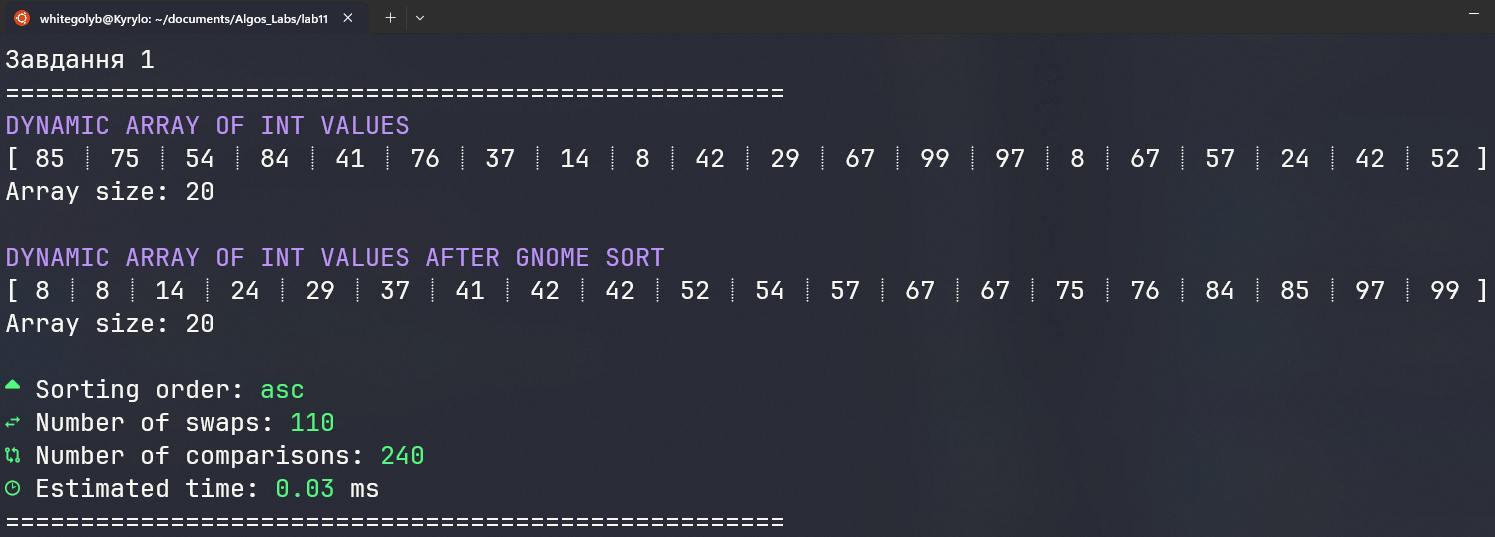
\includegraphics[width=13cm]{reports/algos/lab11/assets/20a.png}
  \caption{Результат для 20 елементів за зростанням}
\end{figure}

\begin{figure}[h!]
  \centering
  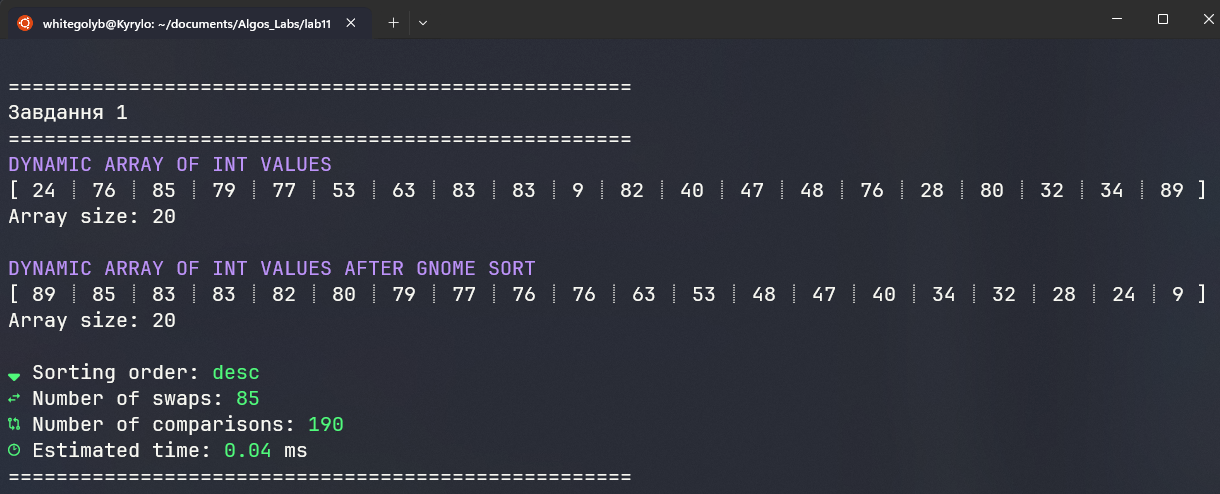
\includegraphics[width=13cm]{reports/algos/lab11/assets/20d.png}
  \caption{Результат для 20 елементів за спаданням}
\end{figure}

\begin{figure}[h!]
  \centering
  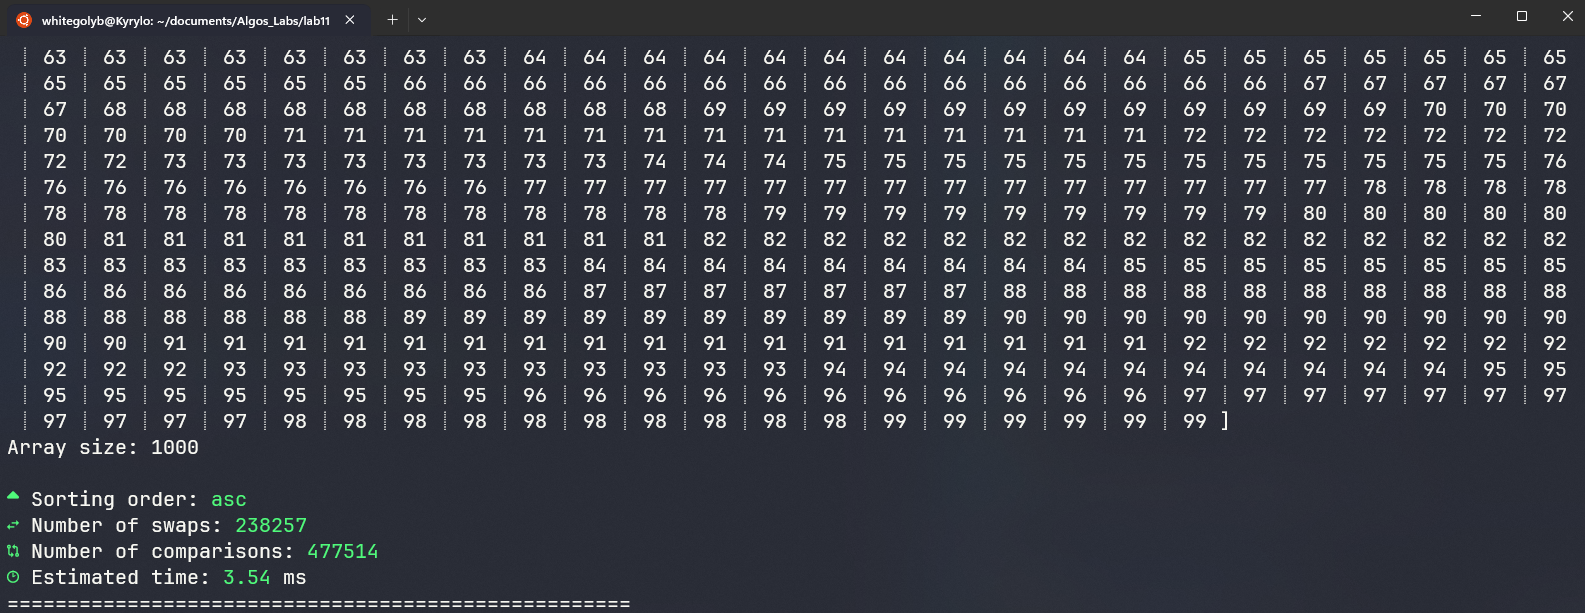
\includegraphics[width=13cm]{reports/algos/lab11/assets/1000a.png}
  \caption{Результат для 1000 елементів за зростанням}
\end{figure}

\begin{figure}[h!]
  \centering
  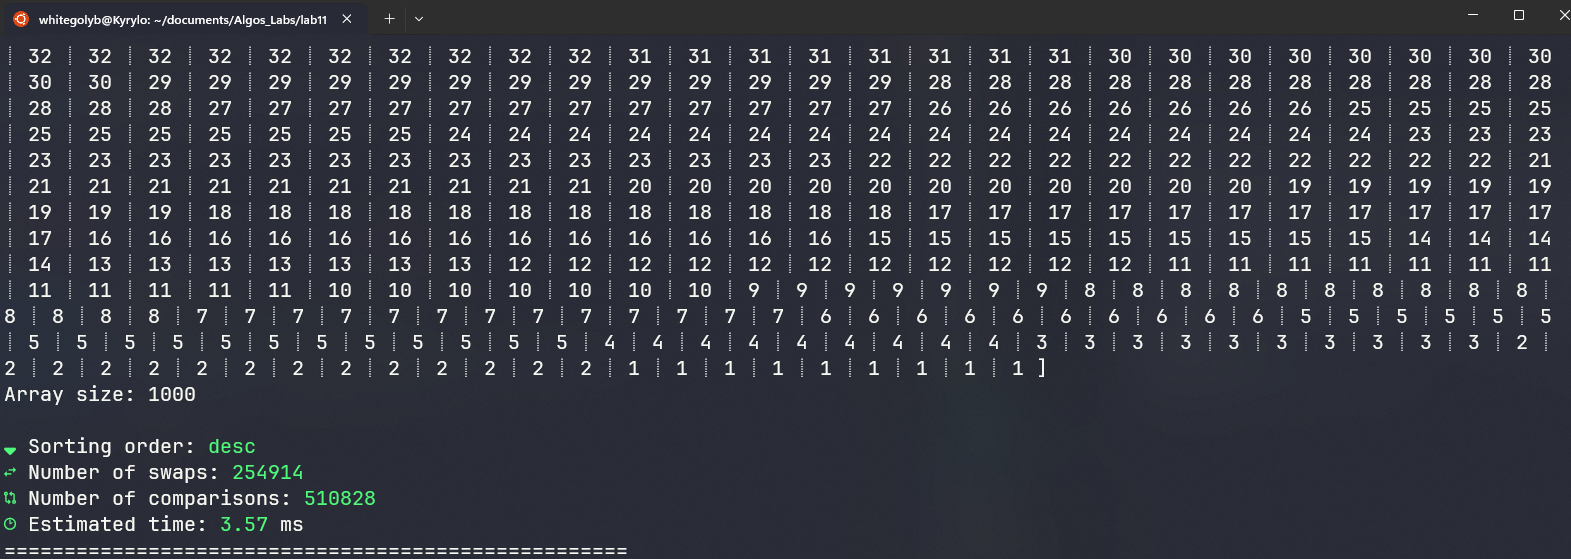
\includegraphics[width=13cm]{reports/algos/lab11/assets/1000d.png}
  \caption{Результат для 1000 елементів за спаданням}
\end{figure}

\begin{figure}[h!]
  \centering
  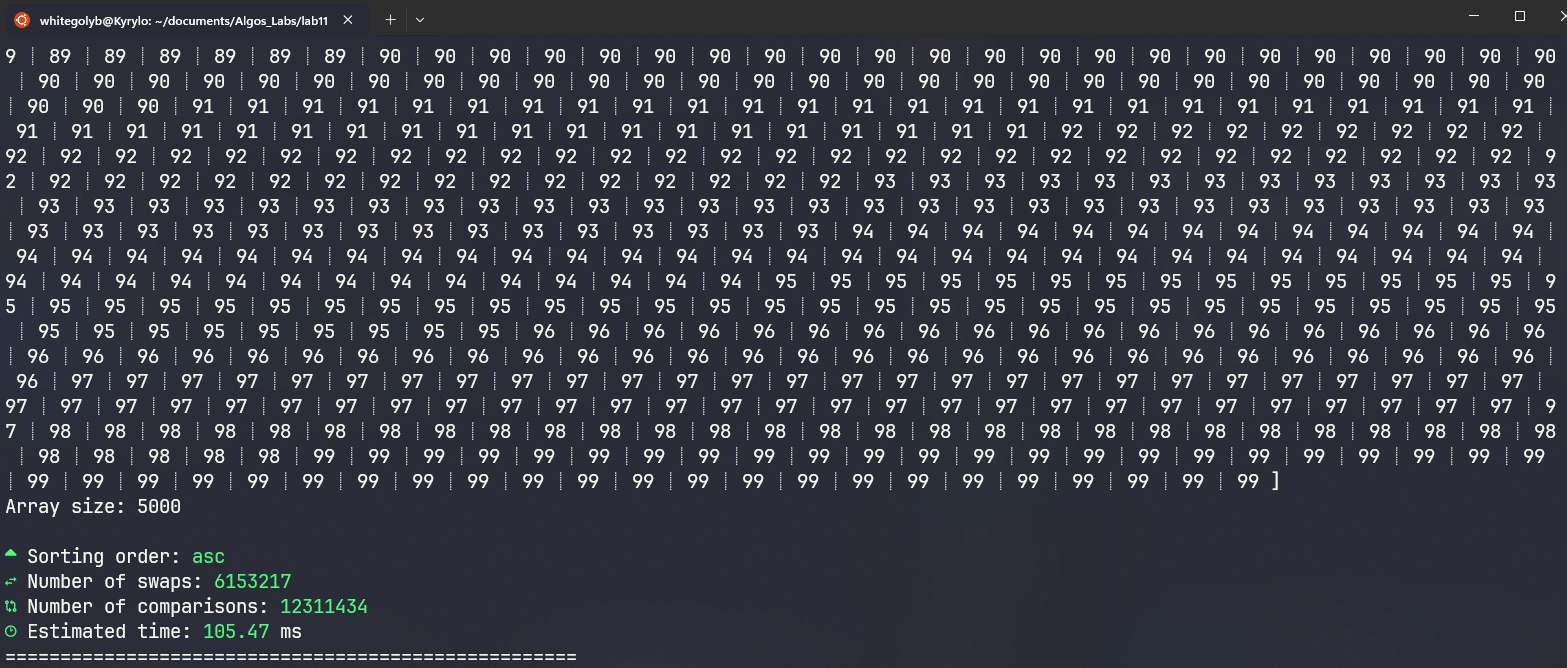
\includegraphics[width=13cm]{reports/algos/lab11/assets/5000a.png}
  \caption{Результат для 5000 елементів за зростанням}
\end{figure}

\begin{figure}[h!]
  \centering
  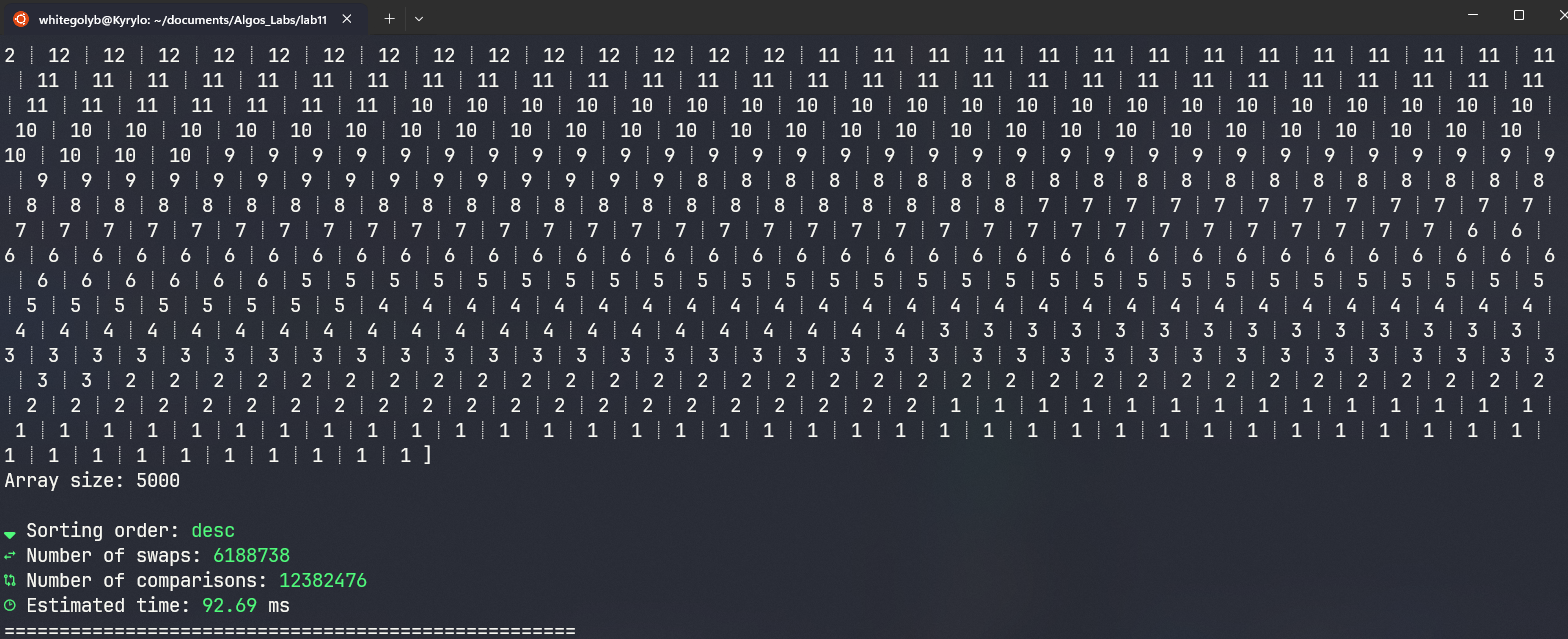
\includegraphics[width=13cm]{reports/algos/lab11/assets/5000d.png}
  \caption{Результат для 5000 елементів за спаданням}
\end{figure}

\begin{figure}[h!]
  \centering
  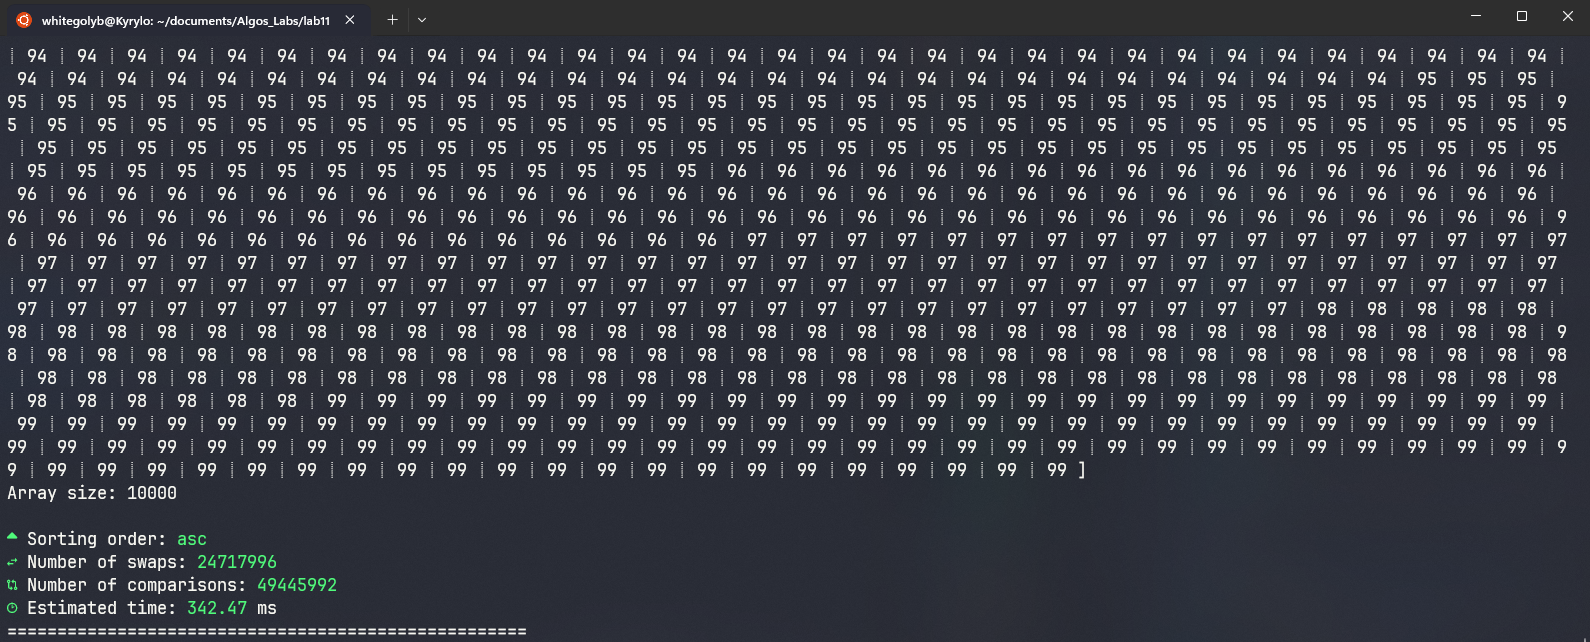
\includegraphics[width=13cm]{reports/algos/lab11/assets/10000a.png}
  \caption{Результат для 10000 елементів за зростанням}
\end{figure}

\begin{figure}[h!]
  \centering
  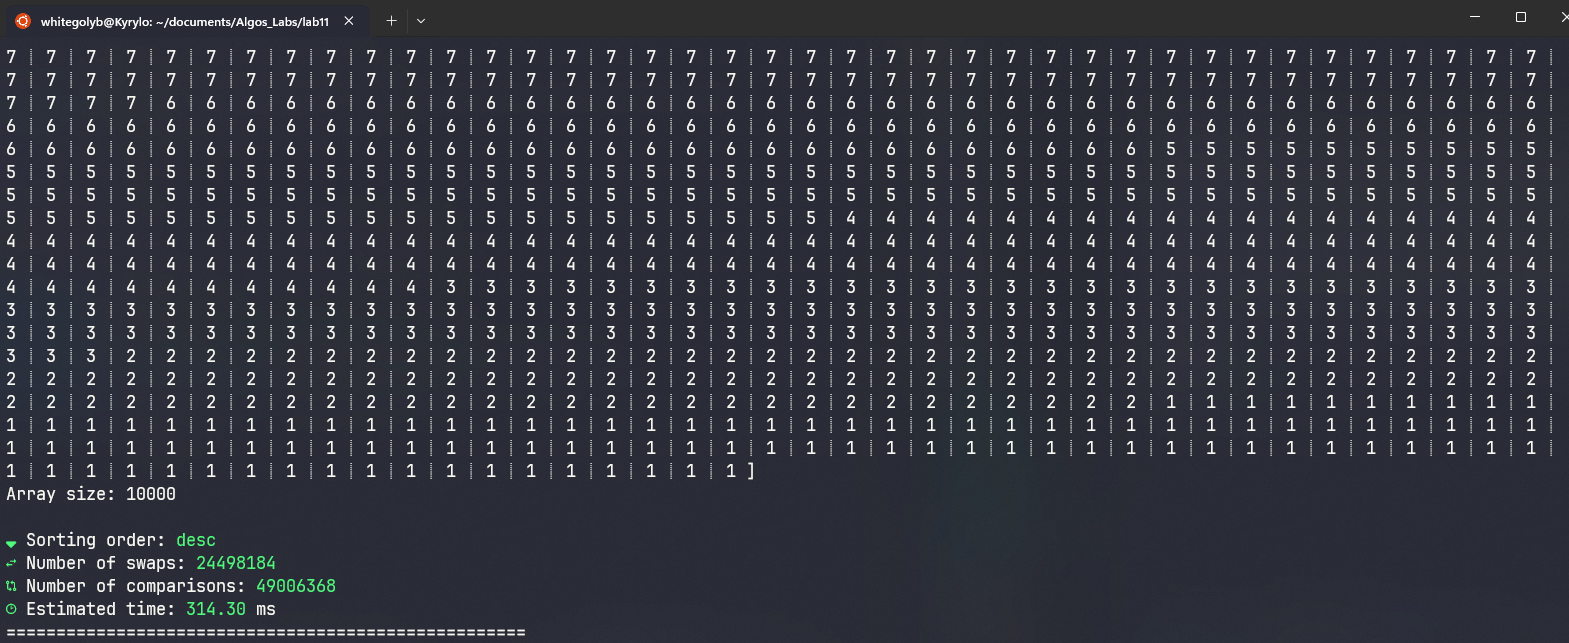
\includegraphics[width=13cm]{reports/algos/lab11/assets/10000d.png}
  \caption{Результат для 10000 елементів за спаданням}
\end{figure}

\begin{figure}[h!]
  \centering
  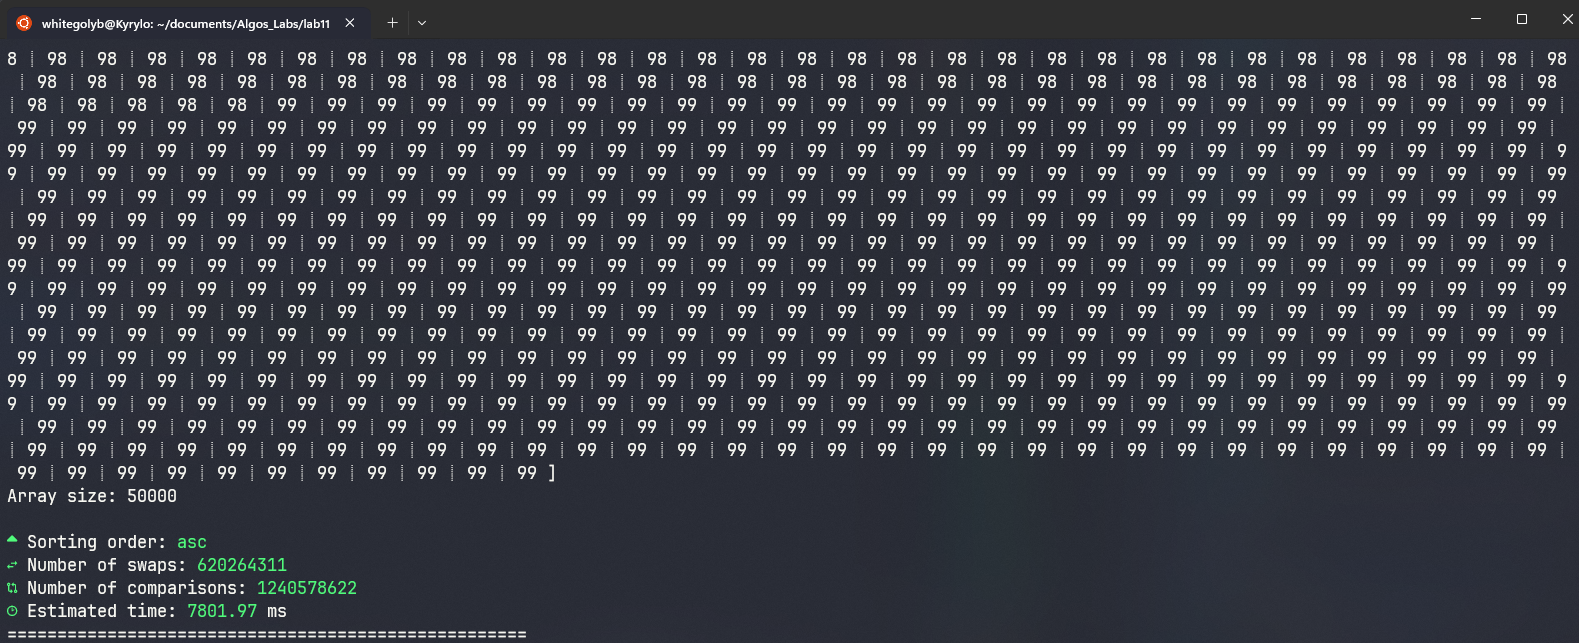
\includegraphics[width=13cm]{reports/algos/lab11/assets/50000a.png}
  \caption{Результат для 50000 елементів за зростанням}
\end{figure}

\begin{figure}[h!]
  \centering
  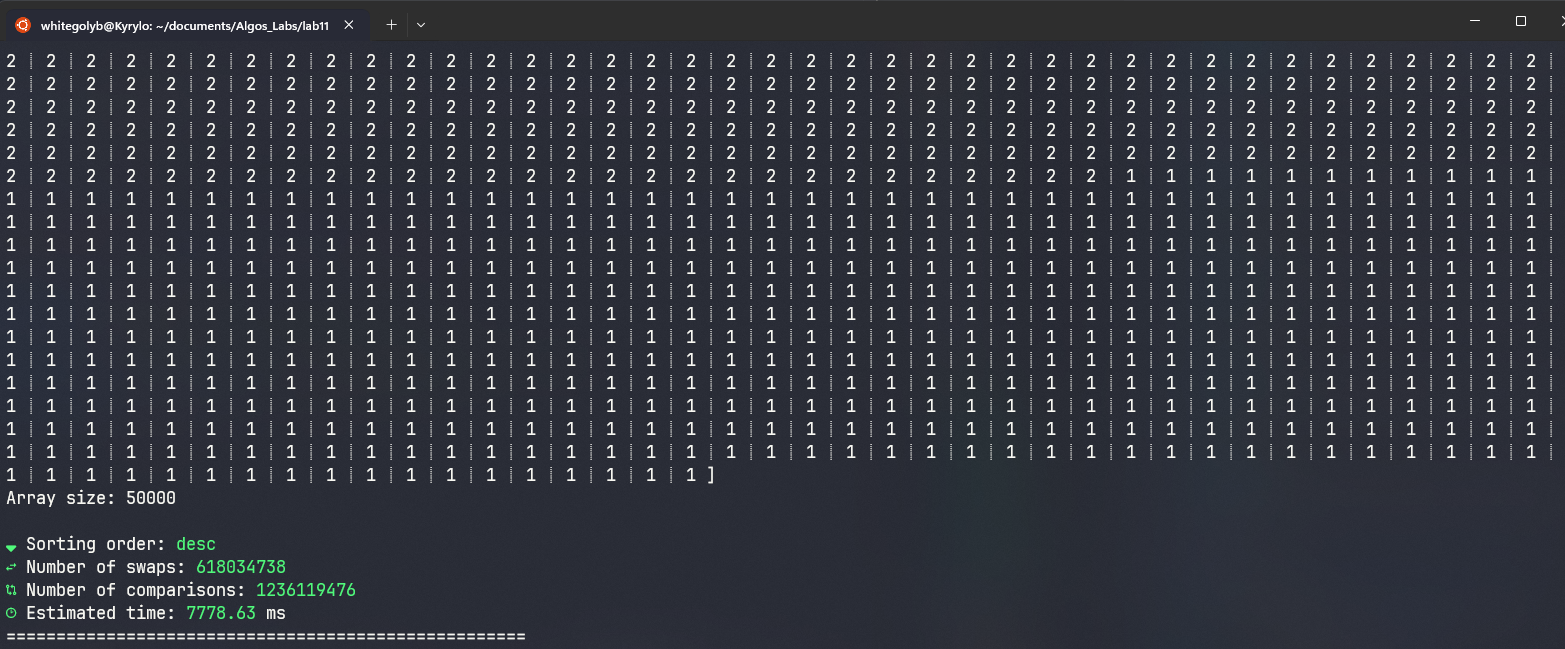
\includegraphics[width=13cm]{reports/algos/lab11/assets/50000d.png}
  \caption{Результат для 50000 елементів за спаданням}
\end{figure}



\clearpage
\subsubsection{Аналіз результатів сортування}

\begin{table}[htbp]
  \caption{Таблиця результатів сортування за зростанням}
  \begin{tabular}{|l|c|c|c|c|c|}
  \hline
  \textit{Відсортований набір даних} & 20   & 1000   & 5000     & 10000    & 50000      \\ \hline
  Кількість пересилань               & 110  & 238257 & 6153217  & 24717996 & 620264311  \\ \hline
  Кількість порівнянь                & 240  & 477514 & 12311434 & 49445992 & 1240578622 \\ \hline
  Час сортування (мс.)               & 0.03 & 3.54   & 105.47   & 342.47   & 7801.97    \\ \hline
  \end{tabular}
\end{table}

\begin{table}[htbp]
  \caption{Таблиця результатів сортування за спаданням}
  \begin{tabular}{|l|c|c|c|c|c|}
  \hline
  \textit{Відсортований набір даних} & 20   & 1000   & 5000     & 10000    & 50000      \\ \hline
  Кількість пересилань               & 85   & 254914 & 6188738  & 24498184 & 618034738  \\ \hline
  Кількість порівнянь                & 190  & 510828 & 12382476 & 49006368 & 1236119476 \\ \hline
  Час сортування (мс.)               & 0.04 & 3.57   & 92.69    & 314.30   & 7778.63    \\ \hline
  \end{tabular}
\end{table}


\clearpage
Графіки побудовані на основі таблиць
\begin{figure}[h!]
  \centering
  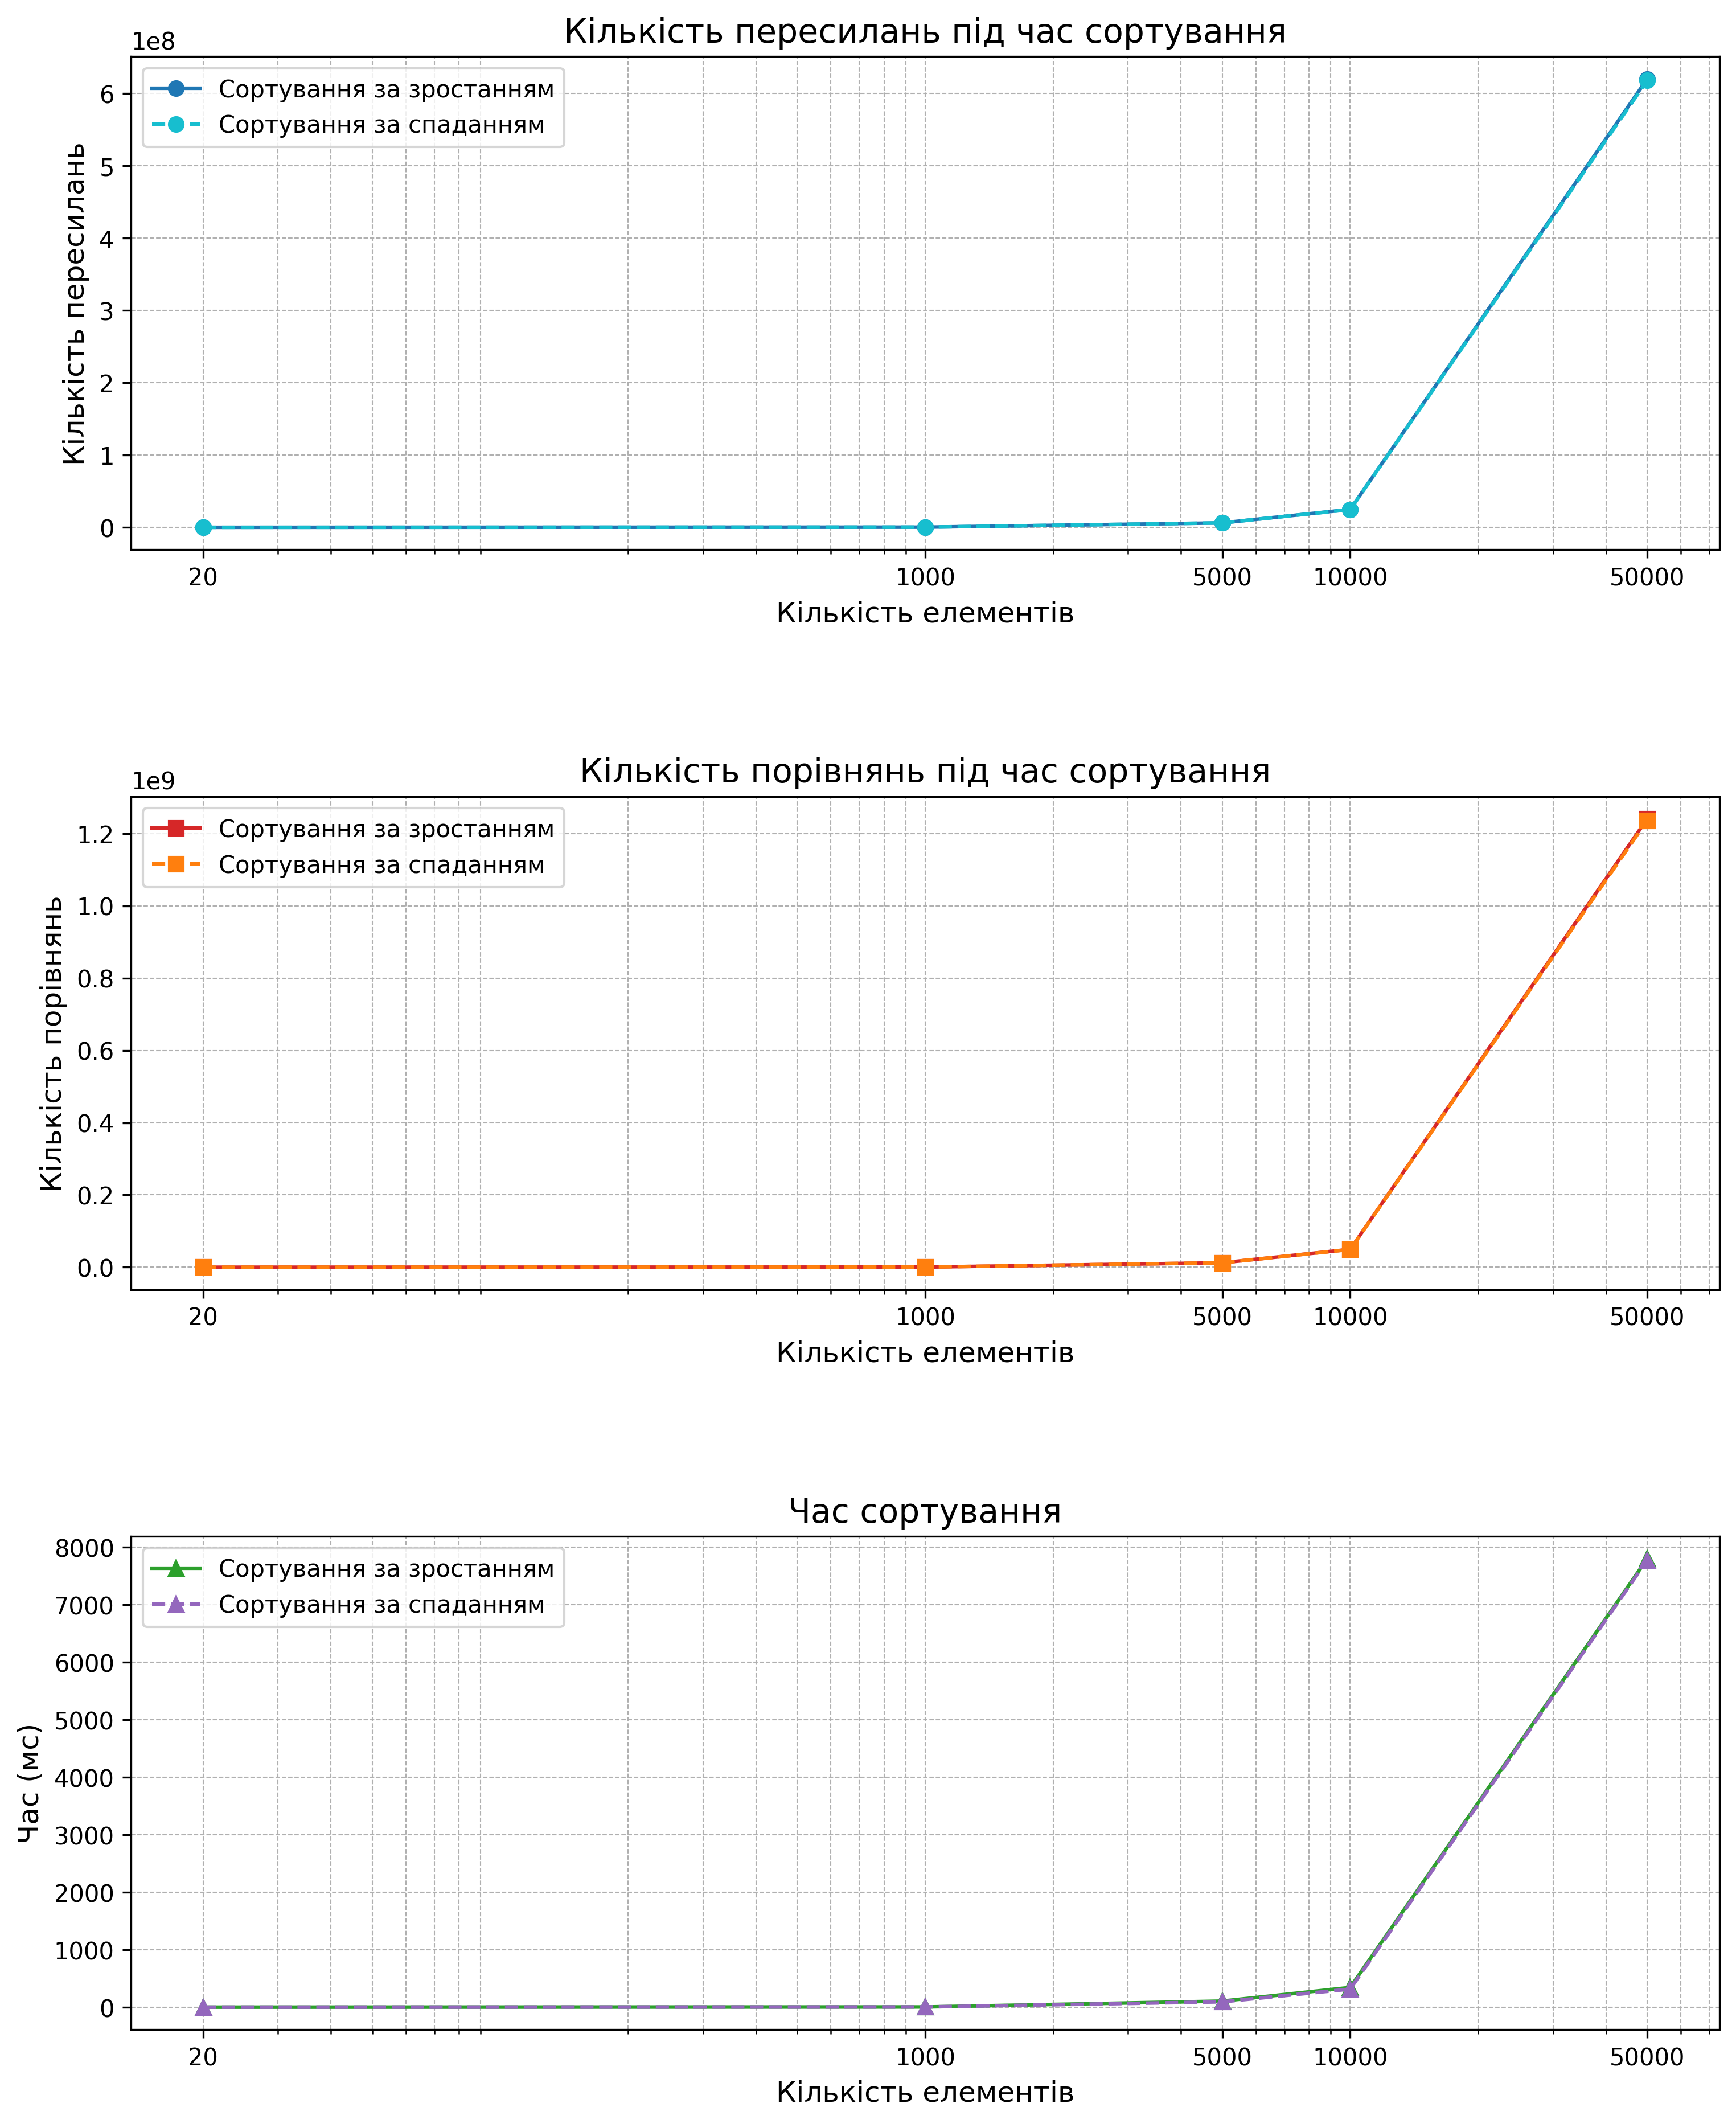
\includegraphics[width=18cm]{reports/algos/lab11/assets/plot.png}
\end{figure}

\clearpage
\section{Висновки}
В ході виконання лабораторної роботи було розроблено метод Гномчого сортування та структуру даних динамічний масив.\\

Після проведення тестування з отриманих результатів були відповідно побудовані графікі залежності часу виконання, кількість порівнянь та пересилань від кількості елементів у масиві. Масив був заповнений випадковими цілими числами.\\

За результатами можна зазначити що сортування значно повільніше починає працювати коли зростає розмір масиву, також сильно зростає кількість порівнянь та пересувань відповідно. Це через те що сам алгоритм має складність  O(n2) у поганому випадку та O(n) у найкращому (коли всі елементи відсортовані).\\

Цей алгоритм не є оптимальним для великих обсягів даних.



